% ============================================================
%  يُترجَم بـ XeLaTeX  (في Overleaf: Menu → Compiler → XeLaTeX)
%  الخط: Amiri (متوفر في Overleaf، أو حمّله من github.com/aliftype/amiri)
% ============================================================
\documentclass[12pt,a4paper]{article}
\usepackage[a4paper,margin=1.7cm,top=2.3cm,bottom=2.9cm,headheight=15pt,footskip=1.5cm]{geometry}
\usepackage{amsmath,amssymb}
\usepackage{icomma}
\usepackage[english,bidi=default,layout=lists]{babel}
\babelprovide[import,main]{arabic}
\babelfont{rm}[Scale=1.08]{Amiri}
\babelfont{sf}[Scale=1.08]{Amiri}
\usepackage[most]{tcolorbox}
\usepackage{tikz}
\usetikzlibrary{arrows.meta,calc,shadings}
\usepackage{array}
\usepackage{colortbl}
\usepackage{fancyhdr}
\usepackage{titlesec}
\usepackage{enumitem}
\usepackage{collcell}
\usepackage{needspace}
\usepackage{etoolbox}
\newcolumntype{C}{>{\collectcell\ar}c<{\endcollectcell}}
\pretocmd{\section}{\Needspace{15\baselineskip}}{}{}
\pretocmd{\subsection}{\Needspace{11\baselineskip}}{}{}

\definecolor{cDef}{HTML}{1F4E9C}
\definecolor{cThm}{HTML}{B3261E}
\definecolor{cRem}{HTML}{2E7D32}
\definecolor{cEx}{HTML}{C76B00}
\definecolor{cMeth}{HTML}{6A1B9A}
\definecolor{cSol}{HTML}{00695C}
\definecolor{cSec}{HTML}{1F3A68}

\titleformat{\section}{\Large\bfseries\color{cSec}}{\thesection.}{0.6em}{}[{\color{cSec!60}\titlerule[1pt]}]
\titleformat{\subsection}{\large\bfseries\color{cThm!85!black}}{\thesubsection.}{0.5em}{}
\titlespacing*{\section}{0pt}{14pt}{8pt}
\titlespacing*{\subsection}{0pt}{10pt}{5pt}
\setlength{\parindent}{0pt}
\setlength{\parskip}{4pt}
\setlist{itemsep=2pt,topsep=3pt}

\newtcolorbox{arbox}[3][]{enhanced,
  colback=#2!5,colframe=#2!80!black,arc=2mm,boxrule=0.8pt,
  left=6pt,right=6pt,top=8pt,bottom=5pt,
  fonttitle=\bfseries,coltitle=white,
  title={\foreignlanguage{arabic}{#3}},
  attach boxed title to top right={xshift=-5mm,yshift=-3mm},
  boxed title style={colback=#2!80!black,arc=1.5mm,boxrule=0pt},
  before upper={\selectlanguage{arabic}},
  before skip=8pt,after skip=8pt,breakable,#1}
\newenvironment{BOX}[2]{\begin{otherlanguage}{english}\begin{arbox}{#1}{#2}}{\end{arbox}\end{otherlanguage}}
\newenvironment{tarif}[1][تعريف]{\begin{BOX}{cDef}{#1}}{\end{BOX}}
\newenvironment{khassia}[1][خاصية]{\begin{BOX}{cThm}{#1}}{\end{BOX}}
\newenvironment{molahada}[1][ملاحظة]{\begin{BOX}{cRem}{#1}}{\end{BOX}}
\newenvironment{mithal}[1][مثال]{\begin{BOX}{cEx}{#1}}{\end{BOX}}
\newenvironment{tariqa}[1][طريقة]{\begin{BOX}{cMeth}{#1}}{\end{BOX}}

\newcounter{exo}
\newenvironment{tamrin}[1]{\stepcounter{exo}\begin{BOX}{cSec}{التمرين \theexo: #1}}{\end{BOX}}
\newenvironment{hal}{\Needspace{12\baselineskip}\begin{otherlanguage}{english}\begin{arbox}[breakable]{cSol}{حل التمرين \theexo}}{\end{arbox}\end{otherlanguage}}

\newenvironment{LTR}{\begin{otherlanguage}{english}}{\end{otherlanguage}}
\newcommand{\ar}[1]{\foreignlanguage{arabic}{#1}}

\renewcommand{\dots}{\mathinner{\ldotp\ldotp\ldotp}}
\renewcommand{\ldots}{\mathinner{\ldotp\ldotp\ldotp}}
\renewcommand{\cdots}{\mathinner{\cdotp\cdotp\cdotp}}
\newcommand{\N}{\mathbb{N}}
\newcommand{\Z}{\mathbb{Z}}
\newcommand{\D}{\mathbb{D}}
\newcommand{\Q}{\mathbb{Q}}
\newcommand{\R}{\mathbb{R}}
\newcommand{\pgcd}{\operatorname{PGCD}}
\newcommand{\ppcm}{\operatorname{PPCM}}

% \NLseg{a}{b}{[}{]} ; \NLright{a}{[} ; \NLleft{b}{]}  (interval on a number line)
\newcommand{\NLseg}[4]{\begin{LTR}\begin{tikzpicture}[baseline=-0.6ex]
 \draw[-{Stealth[length=2mm]},gray!70](0,0)--(3.4,0);
 \draw[line width=2pt,cThm!80!black](0.7,0)--(2.7,0);
 \node[cThm!80!black,font=\LARGE] at (0.7,0){$#3$};
 \node[cThm!80!black,font=\LARGE] at (2.7,0){$#4$};
 \node[below=3pt,font=\footnotesize] at (0.7,0){$#1$};
 \node[below=3pt,font=\footnotesize] at (2.7,0){$#2$};
\end{tikzpicture}\end{LTR}}
\newcommand{\NLright}[2]{\begin{LTR}\begin{tikzpicture}[baseline=-0.6ex]
 \draw[-{Stealth[length=2mm]},gray!70](0,0)--(3.4,0);
 \draw[line width=2pt,cThm!80!black](1.3,0)--(3.3,0);
 \node[cThm!80!black,font=\LARGE] at (1.3,0){$#2$};
 \node[below=3pt,font=\footnotesize] at (1.3,0){$#1$};
\end{tikzpicture}\end{LTR}}
\newcommand{\NLleft}[2]{\begin{LTR}\begin{tikzpicture}[baseline=-0.6ex]
 \draw[-{Stealth[length=2mm]},gray!70](0,0)--(3.4,0);
 \draw[line width=2pt,cThm!80!black](0.05,0)--(2.1,0);
 \node[cThm!80!black,font=\LARGE] at (2.1,0){$#2$};
 \node[below=3pt,font=\footnotesize] at (2.1,0){$#1$};
\end{tikzpicture}\end{LTR}}

% ---------- social-media icons (pure TikZ) ----------
\definecolor{cFB}{HTML}{1877F2}
\definecolor{cTG}{HTML}{229ED9}
\definecolor{cIG1}{HTML}{FEDA75}
\definecolor{cIG2}{HTML}{D62976}
\definecolor{cIG3}{HTML}{4F5BD5}
\newcommand{\fbicon}{\begin{LTR}\begin{tikzpicture}[baseline=-0.75ex,x=1em,y=1em]
 \fill[cFB] (0,0) circle (0.55);
 \node[white,inner sep=0,font=\usefont{TU}{lmss}{bx}{n}\small] at (0.04,-0.02) {f};
\end{tikzpicture}\end{LTR}}
\newcommand{\igicon}{\begin{LTR}
\begin{tikzpicture}[baseline=-0.75ex,x=1em,y=1em]
 \shade[lower left=cIG1,lower right=cIG2,upper left=cIG2,upper right=cIG3,rounded corners=0.28em] (-0.55,-0.55) rectangle (0.55,0.55);
 \draw[white,line width=0.09em,rounded corners=0.18em] (-0.36,-0.36) rectangle (0.36,0.36);
 \draw[white,line width=0.09em] (0,0) circle (0.17);
 \fill[white] (0.22,0.22) circle (0.05);
\end{tikzpicture}\end{LTR}}
\newcommand{\tgicon}{\begin{LTR}
\begin{tikzpicture}[baseline=-0.75ex,x=1em,y=1em]
 \fill[cTG] (0,0) circle (0.55);
 \fill[white] (-0.33,0.0) -- (0.32,0.27) -- (0.2,-0.3) -- (0.0,-0.15) -- (-0.08,-0.28) -- (-0.08,-0.08) -- cycle;
 \fill[cTG!70!black] (-0.08,-0.08) -- (0.25,0.2) -- (0.0,-0.15) -- (-0.08,-0.28) -- cycle;
\end{tikzpicture}\end{LTR}}
% page number: black box, white two-digit number, at the right of the social row
\newcommand{\PageBox}{\begin{LTR}\tikz[baseline=(p.base)]\node[fill=black,text=white,inner sep=2.5pt,minimum width=1.6em,minimum height=1.3em,font=\usefont{TU}{lmss}{bx}{n}\small](p){\ifnum\value{page}<10 0\fi\arabic{page}};\end{LTR}}
% visual left-to-right order: Telegram | Instagram | Facebook | page box
\newcommand{\SocialRow}{\begin{otherlanguage}{english}%
 \ar{\textbf{الأستاذ سوايسية هشام للرياضيات}}\ \tgicon\hfill
 \textbf{prof\_hicham\_math}\ \igicon\hfill
 \ar{\textbf{الأستاذ سوايسية هشام للرياضيات}}\ \fbicon\hspace{2.2em}\PageBox\end{otherlanguage}}

\pagestyle{fancy}
\fancyhf{}
\renewcommand{\headrulewidth}{0.6pt}
\renewcommand{\footrulewidth}{0.4pt}
% \SetHeader{right head: document title}{left head: level -- stream}
\newcommand{\SetHeader}[2]{%
 \fancyhead[C]{\parbox{\textwidth}{\ar{#1\hfill #2}}}%
 \fancyfoot[C]{\parbox{\textwidth}{\small\SocialRow}}}
\usepackage{tkz-tab}
\usepackage{multicol}
% variation / sign table (LTR)
\newenvironment{TAB}{\par\begin{center}\begin{LTR}\begin{tikzpicture}[scale=0.95,every node/.style={font=\small}]}{\end{tikzpicture}\end{LTR}\end{center}}
% grid + axes, clipped: \begin{GR}{xmin}{xmax}{ymin}{ymax}{unit cm}
\newenvironment{GR}[5]{\par\begin{center}\begin{LTR}\begin{tikzpicture}[x=#5cm,y=#5cm,font=\footnotesize]
 \draw[gray!25,very thin] (#1,#3) grid (#2,#4);
 \draw[-{Stealth[length=2mm]}] (#1,0)--(#2+0.3,0) node[below left]{$x$};
 \draw[-{Stealth[length=2mm]}] (0,#3)--(0,#4+0.3) node[below left]{$y$};
 \node[below left] at (0,0){$O$};
 \begin{scope}\clip (#1,#3) rectangle (#2,#4);}
{\end{scope}\end{tikzpicture}\end{LTR}\end{center}}
\newcommand{\Ticks}[2]{\foreach \t in {#1} \node[below,font=\scriptsize] at (\t,0){$\t$}; \foreach \t in {#2} \node[left,font=\scriptsize] at (0,\t){$\t$};}
\newcommand{\bx}[1]{\ensuremath{\colorbox{cDef!12}{$\displaystyle #1$}}}
\newcommand{\TwoCol}[4]{\par\begin{LTR}\noindent\begin{minipage}[t]{#1\textwidth}\selectlanguage{arabic}#2\end{minipage}\hfill\begin{minipage}[t]{#3\textwidth}\selectlanguage{arabic}#4\end{minipage}\end{LTR}\par}
\newcommand{\RL}[4]{\TwoCol{#3}{#4}{#1}{#2}}  % \RL{w1}{right content}{w2}{left content}
\newcommand{\ok}{$\textcolor{cRem}{\checkmark}$}
\newcommand{\limn}{\displaystyle\lim_{n\to+\infty}}
% sub-questions, each on its own line
\newenvironment{sq}{\begin{itemize}[leftmargin=2.4em,itemsep=3pt]}{\end{itemize}}
\newcommand{\qa}{\item[(أ)]}\newcommand{\qb}{\item[(ب)]}\newcommand{\qc}{\item[(جـ)]}\newcommand{\qd}{\item[(د)]}\newcommand{\qe}{\item[(هـ)]}
\newcommand{\pa}{\par\smallskip\textbf{(أ)} }\newcommand{\pb}{\par\smallskip\textbf{(ب)} }\newcommand{\pc}{\par\smallskip\textbf{(جـ)} }\newcommand{\pd}{\par\smallskip\textbf{(د)} }\newcommand{\pe}{\par\smallskip\textbf{(هـ)} }
\newcommand{\QQ}[1]{\par\smallskip\textbf{#1.} }
\newenvironment{tmr}{\stepcounter{exo}\begin{BOX}{cSec}{تمرين محلول \theexo}}{\end{BOX}}
\newcommand{\ABC}[3]{\\[2pt]\begin{tabular}{p{0.28\textwidth}p{0.28\textwidth}p{0.28\textwidth}}(جـ) \ #3 & (ب) \ #2 & (أ) \ #1\end{tabular}}
\pretocmd{\section}{\Needspace{24\baselineskip}}{}{}
\newtcbox{\bxtbox}{on line,colback=cDef!12,colframe=cDef!12,boxrule=0pt,arc=1pt,boxsep=0pt,left=2pt,right=2pt,top=1pt,bottom=1pt}
\newcommand{\bxt}[1]{\foreignlanguage{english}{\bxtbox{\ar{#1}}}}
\usepackage{longtable}
\setlength{\LTpre}{4pt}\setlength{\LTpost}{0pt}
\newcommand{\Phase}[1]{\textbf{#1}}
\newcommand{\Fld}[2]{\textbf{#1:}\ #2}
% رأس المذكرة على نمط النموذج: إطار بعنوان «مذكرة رقم»، معلومات الحصة، ثم إطار الكفاءات
\newcommand{\ModhHead}[9]{%
\begin{LTR}
\begin{tcolorbox}[enhanced,colback=white,colframe=cThm!85!black,arc=4mm,boxrule=1pt,top=14pt,bottom=6pt,left=8pt,right=8pt,
 overlay={\node[fill=cThm!85!black,text=white,rounded corners=3mm,inner xsep=14pt,inner ysep=4pt,font=\large\bfseries] at ([yshift=0pt]frame.north){\ar{مذكرة رقم #1}};},
 before upper={\selectlanguage{arabic}}]
\begin{tabular}{@{}p{0.4\linewidth}p{0.55\linewidth}@{}}
\Fld{المستوى}{#2} & \Fld{الثانوية}{\dotfill}\\[3pt]
\Fld{المادة}{رياضيات} & \Fld{ميدان التعلم}{#3}\\[3pt]
\Fld{المدة}{#5} & \Fld{الوحدة التعلمية}{#4}\\[3pt]
\Fld{الأستاذ}{\dotfill} & \Fld{المحتوى المعرفي}{#6}\\
\end{tabular}
\end{tcolorbox}
\begin{tcolorbox}[enhanced,colback=white,colframe=cThm!85!black,arc=3mm,boxrule=0.8pt,sidebyside,sidebyside align=top,lefthand ratio=0.5,
 segmentation style={dashed,cThm!60},before upper={\selectlanguage{arabic}},before lower={\selectlanguage{arabic}}]
\textbf{الكفاءات المستهدفة:}\par #8
\tcblower
\textbf{الكفاءات القبلية:}\par #7
\end{tcolorbox}
\end{LTR}
\par\smallskip\textbf{الوسائل:} #9\par\smallskip}
\newenvironment{Sayr}{%
\begin{LTR}\renewcommand{\arraystretch}{1.25}
\begin{longtable}{|p{0.17\textwidth}|>{\centering\arraybackslash}p{0.06\textwidth}|p{0.53\textwidth}|>{\centering\arraybackslash}p{0.12\textwidth}|}
\hline\rowcolor{cThm!12}\ar{\textbf{توجيهات وتعاليق}} & \ar{\textbf{المدة}} & \ar{\textbf{سير الحصة}} & \ar{\textbf{مراحل الحصة}}\\\hline\endhead
\hline\endfoot}{\end{longtable}\end{LTR}}
% سطر في الجدول: \Row{مرحلة}{سير}{مدة}{توجيهات}
\newcommand{\Row}[4]{\ar{\small #4} & \ar{#3} & \ar{#2} & \cellcolor{cThm!8}\ar{\Phase{#1}}\\\hline}

\newcommand{\Lab}[2]{\foreignlanguage{english}{\tcbox[on line,colback=#1,colframe=#1,boxrule=0pt,arc=2pt,boxsep=1pt,left=5pt,right=5pt,top=1pt,bottom=1pt]{\ar{\textcolor{white}{\textbf{#2}}}}}}
\newcommand{\Num}[1]{\foreignlanguage{english}{\tikz[baseline=(c.base)]\node[fill=cDef,text=white,inner sep=2pt,font=\footnotesize\bfseries](c){#1};}}
\newcommand{\ck}{\ensuremath{{\color{cRem}\checkmark}}}
\newenvironment{Kad}[1]{\par\smallskip\Lab{#1}}{\par}
\SetHeader{\small\bfseries\color{cSec}مذكرات محور: الجداء السلمي في المستوي}{\small\color{cSec}السنة الثانية ثانوي -- علوم تجريبية}
\begin{document}
\begin{LTR}
\begin{tcolorbox}[enhanced,colback=cThm!85!black,colframe=cThm!85!black,arc=3mm,halign=center,boxrule=0pt,top=12pt,bottom=12pt,before upper={\selectlanguage{arabic}}]
{\color{white}\fontsize{24}{30}\selectfont\bfseries مذكرات محور: الجداء السلمي في المستوي}\\[8pt]
{\color{white}\large السنة الثانية ثانوي -- علوم تجريبية (صالحة لشعبتي رياضيات وتقني رياضي)}\\[4pt]
{\color{white}\large 8 مذكرات (16 ساعة) -- السنة الدراسية 2026-2027}
\end{tcolorbox}
\end{LTR}
\begin{BOX}{cThm}{يتضمن هذا العمل}
\begin{enumerate}[label=\textbf{مذكرة \arabic{enumi}:},leftmargin=6em,start=48]
\item الجداء السلمي: تعريفه وحسابه.
\item خواص الجداء السلمي والتعامد.
\item معادلة مستقيم بشعاع ناظمي ، معادلة دائرة.
\item المسافة بين نقطة ومستقيم.
\item العلاقات المترية في المثلث: الكاشي ، المتوسط ، المساحة.
\item تعيين مجموعات نقط باستعمال الجداء السلمي.
\item دساتير الجمع والتضعيف.
\item حل المعادلة $a\cos x+b\sin x=c$.
\end{enumerate}
مراجع النشاطات والتمارين: الكتاب المدرسي للسنة الثانية ثانوي (باب الجداء السلمي).
\end{BOX}
\newpage
\ModhHead{48}{2 ع ت}{هندسة}{الجداء السلمي في المستوي}{02 سا}{الجداء السلمي: تعريفه وحسابه}%
{\begin{itemize}\item الأشعة ، الإسقاط العمودي ، جيب التمام ، مبرهنة فيثاغورس.\end{itemize}}%
{\begin{itemize}\item حساب الجداء السلمي لشعاعين بطرق مختلفة.\end{itemize}}%
{المنهاج ، الكتاب المدرسي ، مراجع ، الحاسبة ، أدوات الهندسة.}
\begin{Sayr}
\Row{مرحلة الانطلاق}{%
\textbf{التهيئة النفسية:} مبرهنة فيثاغورس صحيحة في المثلث القائم: ماذا يحدث للعدد $AB^2+AC^2-BC^2$ إذا لم يكن المثلث قائماً؟}{10 د}{سؤال تمهيدي.}
\Row{التشخيص والاكتشاف}{%
\Lab{cEx}{مناقشة نشاط 01 (أنشطة باب الجداء السلمي)}\par\ck\ $H$ المسقط العمودي لـ $C$ على $(AB)$: ثلاث وضعيات للنقطة $H$.\par
\ck\ نجد أن $\frac12(AB^2+AC^2-BC^2)$ يساوي $AB\times AH$ بإشارة حسب الوضعية: هذا العدد هو \textbf{الجداء السلمي} $\overrightarrow{AB}\cdot\overrightarrow{AC}$.\par
}{35 د}{ثلاث وضعيات للمسقط.}
\Row{بناء المعارف}{%
\Lab{cDef}{تعريف}\ $\vec u\cdot\vec v=\|\vec u\|\,\|\vec v\|\cos(\vec u;\vec v)$ (ويساوي $0$ إذا كان أحدهما معدوماً).\par\Lab{cThm}{طرق الحساب}\par\ck\ \textbf{بالإسقاط}: $\overrightarrow{AB}\cdot\overrightarrow{AC}=\overrightarrow{AB}\cdot\overrightarrow{AH}$ ($H$ مسقط $C$ على $(AB)$).\par
\ck\ \textbf{بالنظيمين}: $\vec u\cdot\vec v=\frac12\left(\|\vec u+\vec v\|^2-\|\vec u\|^2-\|\vec v\|^2\right)$.\par
\ck\ \textbf{بالمركبات} (معلم متعامد ومتجانس): $\vec u(x;y)$ ، $\vec v(x^{\prime};y^{\prime})$: $\vec u\cdot\vec v=xx^{\prime}+yy^{\prime}$.\par
\par\smallskip\begin{LTR}\centering 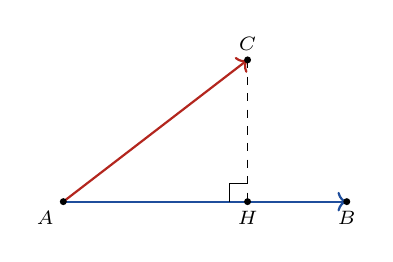
\begin{tikzpicture}[scale=0.9,font=\scriptsize]
\coordinate (A) at (0,0); \coordinate (B) at (4,0); \coordinate (C) at (2.6,2); \coordinate (H) at (2.6,0);
\draw[thick,->,cDef] (A)--(B); \draw[thick,->,cThm] (A)--(C); \draw[dashed] (C)--(H);
\draw (2.6,0.25)--(2.35,0.25)--(2.35,0);
\fill (A) circle (1.4pt) node[below left]{$A$}; \fill (B) circle (1.4pt) node[below]{$B$};
\fill (C) circle (1.4pt) node[above]{$C$}; \fill (H) circle (1.4pt) node[below]{$H$};
\end{tikzpicture}\end{LTR}\par }{50 د}{الطرق الثلاث في جدول.}
\Row{}{%
\Lab{cEx}{مثال}\ $AB=4$ ، $AC=3$ ، $\widehat{BAC}=\frac\pi3$: $\overrightarrow{AB}\cdot\overrightarrow{AC}=4\times3\times\frac12=6$ ؛ $\vec u(2;-1)$ ، $\vec v(3;4)$: $\vec u\cdot\vec v=6-4=2$.\par\Lab{cThm!80!black}{حذار}\ الجداء السلمي \textbf{عدد} وليس شعاعاً.}{}{}
\Row{التقويم}{%
\Lab{cEx}{تطبيق}\par $ABC$ متقايس الأضلاع طول ضلعه $2$: احسب $\overrightarrow{AB}\cdot\overrightarrow{AC}$. ثم احسب $\vec u\cdot\vec v$ حيث $\vec u(1;2)$ و $\vec v(-4;2)$.\par\textbf{الحل:} $2\times2\times\cos\frac\pi3=2$ ؛ $-4+4=0$.\par\textbf{واجب منزلي:} تمارين 27 ، 29 ، 31 ، 33 ، 34 ، 50 ، 51 من باب الجداء السلمي.\par\smallskip\textbf{ملاحظات حول سير الحصة:} \dotfill}{25 د}{تقويم فردي.}
\end{Sayr}
\newpage
\ModhHead{49}{2 ع ت}{هندسة}{الجداء السلمي في المستوي}{02 سا}{خواص الجداء السلمي والتعامد}%
{\begin{itemize}\item تعريف الجداء السلمي وحسابه.\end{itemize}}%
{\begin{itemize}\item استعمال خواص الجداء السلمي ، وإثبات تعامد شعاعين أو مستقيمين.\end{itemize}}%
{المنهاج ، الكتاب المدرسي ، مراجع ، الحاسبة ، أدوات الهندسة.}
\begin{Sayr}
\Row{مرحلة الانطلاق}{%
\textbf{التهيئة النفسية:} إذا كان $\vec u\cdot\vec v=0$ ، ماذا نستنتج عن الشعاعين؟}{10 د}{سؤال.}
\Row{التشخيص والاكتشاف}{%
\Lab{cEx}{وضعية مقترحة}\par\ck\ نحسب $(\vec u+\vec v)\cdot(\vec u-\vec v)$ بالنشر: $\|\vec u\|^2-\|\vec v\|^2$.\par
\ck\ في معين: قطراه $\vec u+\vec v$ و $\vec u-\vec v$ وضلعاه متقايسان ، إذن القطران متعامدان.\par
}{35 د}{برهان خاصية المعين.}
\Row{بناء المعارف}{%
\Lab{cThm}{خاصية}\par\ck\ $\vec u\cdot\vec v=\vec v\cdot\vec u$ ؛ $\vec u\cdot(\vec v+\vec w)=\vec u\cdot\vec v+\vec u\cdot\vec w$ ؛ $(k\vec u)\cdot\vec v=k(\vec u\cdot\vec v)$.\par
\ck\ $\vec u^2=\|\vec u\|^2$ ؛ $(\vec u+\vec v)^2=\|\vec u\|^2+2\,\vec u\cdot\vec v+\|\vec v\|^2$.\par
\Lab{cThm}{التعامد}\ $\vec u\perp\vec v$ إذا وفقط إذا كان $\vec u\cdot\vec v=0$.\par}{50 د}{المتطابقات تُحفظ.}
\Row{}{%
\Lab{cEx}{مثال}\ $\|\vec u\|=3$ ، $\|\vec v\|=2$ ، $\vec u\cdot\vec v=-1$: $\|\vec u+\vec v\|^2=9-2+4=11$.\par\Lab{cThm!80!black}{حذار}\ لا يوجد «اختزال»: $\vec u\cdot\vec v=\vec u\cdot\vec w$ لا يعني $\vec v=\vec w$.}{}{}
\Row{التقويم}{%
\Lab{cEx}{تطبيق}\par $A(1;1)$ ، $B(4;2)$ ، $C(0;4)$. بيّن أن المثلث $ABC$ قائم في $A$.\par\textbf{الحل:} $\overrightarrow{AB}(3;1)$ ، $\overrightarrow{AC}(-1;3)$: $\overrightarrow{AB}\cdot\overrightarrow{AC}=-3+3=0$.\par\textbf{واجب منزلي:} تمارين 32 ، 35 ، 36 ، 38 ، 48 ، 59 من باب الجداء السلمي.\par\smallskip\textbf{ملاحظات حول سير الحصة:} \dotfill}{25 د}{تقويم فردي.}
\end{Sayr}
\newpage
\ModhHead{50}{2 ع ت}{هندسة}{الجداء السلمي في المستوي}{02 سا}{معادلة مستقيم بشعاع ناظمي ، معادلة دائرة}%
{\begin{itemize}\item معادلة مستقيم (1 ج م) ، الجداء السلمي بالمركبات.\end{itemize}}%
{\begin{itemize}\item كتابة معادلة مستقيم علم شعاع ناظمي له ونقطة منه.\item كتابة معادلة دائرة وتعيين مركز ونصف قطر دائرة من معادلتها.\end{itemize}}%
{المنهاج ، الكتاب المدرسي ، مراجع ، الحاسبة ، أدوات الهندسة.}
\begin{Sayr}
\Row{مرحلة الانطلاق}{%
\textbf{التهيئة النفسية:} ما مجموعة النقط $M$ حيث $\overrightarrow{AM}\cdot\vec n=0$ ؟}{10 د}{سؤال.}
\Row{التشخيص والاكتشاف}{%
\Lab{cEx}{وضعية مقترحة}\ $A(1;2)$ و $\vec n(3;-1)$.\par\ck\ $M(x;y)$: $\overrightarrow{AM}\cdot\vec n=3(x-1)-(y-2)=0$ ، أي $3x-y-1=0$: مستقيم يشمل $A$ ويعامد $\vec n$.\par
}{35 د}{الحساب بالمركبات.}
\Row{بناء المعارف}{%
\Lab{cThm}{خاصية}\ المستقيم الذي معادلته $ax+by+c=0$ له الشعاع الناظمي $\vec n(a;b)$ ، وشعاع توجيه $(-b;a)$.\par\Lab{cThm}{معادلة دائرة}\ الدائرة التي مركزها $\Omega(a;b)$ ونصف قطرها $r$: $(x-a)^2+(y-b)^2=r^2$.\par}{50 د}{إكمال المربع خطوة خطوة.}
\Row{}{%
\Lab{cEx}{مثال}\par\ck\ $x^2+y^2-4x+6y-3=0$ يكافئ $(x-2)^2+(y+3)^2=16$: دائرة مركزها $(2;-3)$ ونصف قطرها $4$.\par
\ck\ الدائرة ذات القطر $[AB]$: مجموعة النقط $M$ حيث $\overrightarrow{MA}\cdot\overrightarrow{MB}=0$.\par
\Lab{cThm!80!black}{حذار}\ معادلة من الشكل $x^2+y^2+\ldots=k$ قد لا تمثل دائرة إذا كان الطرف الأيمن سالباً بعد الإكمال.}{}{}
\Row{التقويم}{%
\Lab{cEx}{تطبيق}\par اكتب معادلة الدائرة ذات القطر $[AB]$ حيث $A(1;0)$ و $B(3;4)$.\par\textbf{الحل:} المركز $(2;2)$ ، نصف القطر $\frac{AB}2=\sqrt5$: $(x-2)^2+(y-2)^2=5$.\par\textbf{واجب منزلي:} تمارين 62 ، 64 ، 65 ، 68 ، 69 ، 70 ، 75 من باب الجداء السلمي.\par\smallskip\textbf{ملاحظات حول سير الحصة:} \dotfill}{25 د}{تقويم فردي.}
\end{Sayr}
\newpage
\ModhHead{51}{2 ع ت}{هندسة}{الجداء السلمي في المستوي}{02 سا}{المسافة بين نقطة ومستقيم}%
{\begin{itemize}\item الشعاع الناظمي ، معادلة دائرة.\end{itemize}}%
{\begin{itemize}\item حساب المسافة بين نقطة ومستقيم ، وتطبيقها (دائرة مماسة لمستقيم).\end{itemize}}%
{المنهاج ، الكتاب المدرسي ، مراجع ، الحاسبة ، أدوات الهندسة.}
\begin{Sayr}
\Row{مرحلة الانطلاق}{%
\textbf{التهيئة النفسية:} ما أقصر طريق من نقطة إلى طريق مستقيم؟}{10 د}{سؤال من الحياة.}
\Row{التشخيص والاكتشاف}{%
\Lab{cEx}{مناقشة أعمال موجهة (باب الجداء السلمي)}\par\ck\ $H$ المسقط العمودي لـ $A$ على $(D)$: $AH$ أصغر مسافة.\par
\ck\ نستعمل الجداء السلمي $\overrightarrow{HA}\cdot\vec n$ لحساب $AH$.\par
}{35 د}{أعمال موجهة.}
\Row{بناء المعارف}{%
\Lab{cThm}{خاصية}\ المسافة بين $A(x_0;y_0)$ والمستقيم $(D):ax+by+c=0$: $d(A;(D))=\dfrac{|ax_0+by_0+c|}{\sqrt{a^2+b^2}}$.\par\Lab{cEx}{مثال}\ $A(2;1)$ و $(D):3x+4y-5=0$: $d=\dfrac{|6+4-5|}5=1$.\par}{50 د}{الدستور يُحفظ.}
\Row{}{%
\Lab{cThm}{المماس}\ الدائرة التي مركزها $\Omega$ ونصف قطرها $r$ تمس $(D)$ إذا وفقط إذا كان $d(\Omega;(D))=r$.\par\Lab{cThm!80!black}{حذار}\ لا ننسى القيمة المطلقة في البسط.}{}{}
\Row{التقويم}{%
\Lab{cEx}{تطبيق}\par اكتب معادلة الدائرة التي مركزها $\Omega(1;-2)$ وتمس المستقيم $x-y+1=0$.\par\textbf{الحل:} $r=\dfrac{|1+2+1|}{\sqrt2}=2\sqrt2$: $(x-1)^2+(y+2)^2=8$.\par\textbf{واجب منزلي:} تمارين 71 ، 72 ، 73 ، 74 من باب الجداء السلمي.\par\smallskip\textbf{ملاحظات حول سير الحصة:} \dotfill}{25 د}{تقويم فردي.}
\end{Sayr}
\newpage
\ModhHead{52}{2 ع ت}{هندسة}{الجداء السلمي في المستوي}{02 سا}{العلاقات المترية في المثلث: الكاشي ، المتوسط ، المساحة}%
{\begin{itemize}\item الجداء السلمي ، جيب التمام والجيب.\end{itemize}}%
{\begin{itemize}\item حساب أطوال وأقياس زوايا ومساحات باستعمال العلاقات المترية.\end{itemize}}%
{المنهاج ، الكتاب المدرسي ، مراجع ، الحاسبة ، أدوات الهندسة.}
\begin{Sayr}
\Row{مرحلة الانطلاق}{%
\textbf{التهيئة النفسية:} نعرف ضلعين في مثلث والزاوية بينهما: هل نستطيع حساب الضلع الثالث؟}{10 د}{سؤال.}
\Row{التشخيص والاكتشاف}{%
\Lab{cEx}{مناقشة النشاطين 02 و 04 (أنشطة باب الجداء السلمي)}\par\ck\ $\overrightarrow{BC}=\overrightarrow{AC}-\overrightarrow{AB}$ ، نربع: $BC^2=AC^2+AB^2-2\,\overrightarrow{AB}\cdot\overrightarrow{AC}$.\par
\ck\ مساحة مثلث متساوي الساقين بدلالة ضلعه والزاوية.\par
}{35 د}{نشاطا الكتاب.}
\Row{بناء المعارف}{%
\Lab{cThm}{مبرهنة الكاشي}\ $a^2=b^2+c^2-2bc\cos\widehat A$.\par\Lab{cThm}{مبرهنة المتوسط}\ $I$ منتصف $[AB]$: $MA^2+MB^2=2MI^2+\dfrac{AB^2}2$.\par}{50 د}{الحاسبة لقيس الزاوية.}
\Row{}{%
\Lab{cThm}{المساحة}\ $S=\frac12\,bc\sin\widehat A$.\par\Lab{cEx}{مثال}\ $AB=5$ ، $AC=3$ ، $\widehat A=\frac{2\pi}3$: $BC^2=25+9-2\times15\times(-\frac12)=49$ ، $BC=7$ ؛ $S=\frac12\times15\times\frac{\sqrt3}2=\frac{15\sqrt3}4$.\par}{}{}
\Row{}{%
\Lab{cThm!80!black}{حذار}\ $\cos\widehat A<0$ إذا كانت الزاوية منفرجة.}{}{}
\Row{التقويم}{%
\Lab{cEx}{تطبيق}\par مثلث أطوال أضلاعه $4$ ، $5$ ، $6$. احسب جيب تمام الزاوية المقابلة للضلع $6$ ، ثم مساحة المثلث.\par\textbf{الحل:} $\cos\widehat C=\dfrac{16+25-36}{40}=\dfrac18$ ؛ $\sin\widehat C=\dfrac{\sqrt{63}}8$ ؛ $S=\frac12\times4\times5\times\dfrac{3\sqrt7}8=\dfrac{15\sqrt7}4\approx9{,}92$.\par\textbf{واجب منزلي:} تمارين 97 ، 102 إلى 106 من باب الجداء السلمي.\par\smallskip\textbf{ملاحظات حول سير الحصة:} \dotfill}{25 د}{تقويم فردي.}
\end{Sayr}
\newpage
\ModhHead{53}{2 ع ت}{هندسة}{الجداء السلمي في المستوي}{02 سا}{تعيين مجموعات نقط باستعمال الجداء السلمي}%
{\begin{itemize}\item العلاقات المترية ، معادلة دائرة ومستقيم.\end{itemize}}%
{\begin{itemize}\item تعيين وإنشاء مجموعات نقط معرفة بجداء سلمي أو بمجموع مربعات مسافات.\end{itemize}}%
{المنهاج ، الكتاب المدرسي ، مراجع ، الحاسبة ، أدوات الهندسة.}
\begin{Sayr}
\Row{مرحلة الانطلاق}{%
\textbf{التهيئة النفسية:} ما مجموعة النقط $M$ التي ترى منها القطعة $[AB]$ بزاوية قائمة؟}{10 د}{سؤال هندسي.}
\Row{التشخيص والاكتشاف}{%
\Lab{cEx}{وضعية مقترحة}\par\ck\ $\widehat{AMB}$ قائمة يعني $\overrightarrow{MA}\cdot\overrightarrow{MB}=0$: الدائرة ذات القطر $[AB]$ (ماعدا $A$ و $B$ للزاوية).\par
}{35 د}{نرسم المجموعات بـ GeoGebra.}
\Row{بناء المعارف}{%
\Lab{cMeth}{طريقة}\par\ck\ $\overrightarrow{MA}\cdot\overrightarrow{MB}=k$: نُدخل المنتصف $I$: $\overrightarrow{MA}\cdot\overrightarrow{MB}=MI^2-\dfrac{AB^2}4$.\par
\ck\ $MA^2+MB^2=k$: مبرهنة المتوسط ، فنحصل على $MI^2=\ldots$\par
\ck\ $\overrightarrow{AB}\cdot\overrightarrow{AM}=k$: بالإسقاط ، مستقيم عمودي على $(AB)$.\par
\Lab{cEx}{مثال}\ $AB=4$: $MA^2+MB^2=26$ يكافئ $2MI^2+8=26$ ، $MI=3$: دائرة مركزها $I$ ونصف قطرها $3$.\par}{50 د}{جدول الحالات الثلاث.}
\Row{}{%
\Lab{cThm!80!black}{حذار}\ إذا كان $MI^2$ سالباً فالمجموعة خالية.}{}{}
\Row{التقويم}{%
\Lab{cEx}{تطبيق}\par $AB=6$. عيّن: \Num{1} مجموعة النقط $M$ حيث $MA^2+MB^2=50$ ؛ \Num{2} مجموعة النقط $M$ حيث $\overrightarrow{AB}\cdot\overrightarrow{AM}=12$.\par\textbf{الحل:} \Num{1} $2MI^2+18=50$ ، $MI=4$: دائرة ؛ \Num{2} $6\times AH=12$ ، $AH=2$ ($H$ على $[AB]$): المستقيم العمودي على $(AB)$ في $H$.\par\textbf{واجب منزلي:} تمارين 84 إلى 93 من باب الجداء السلمي.\par\smallskip\textbf{ملاحظات حول سير الحصة:} \dotfill}{25 د}{تقويم فردي.}
\end{Sayr}
\newpage
\ModhHead{54}{2 ع ت}{هندسة}{الجداء السلمي في المستوي}{02 سا}{دساتير الجمع والتضعيف}%
{\begin{itemize}\item الجداء السلمي ، الدائرة المثلثية ، الزوايا المرفقة.\end{itemize}}%
{\begin{itemize}\item إثبات دساتير الجمع واستنتاج الدساتير المرتبطة بها ، وحساب قيم مضبوطة.\end{itemize}}%
{المنهاج ، الكتاب المدرسي ، مراجع ، الحاسبة ، أدوات الهندسة.}
\begin{Sayr}
\Row{مرحلة الانطلاق}{%
\textbf{التهيئة النفسية:} هل $\cos\left(\frac\pi3-\frac\pi4\right)=\cos\frac\pi3-\cos\frac\pi4$ ؟ تحقق بالحاسبة.}{10 د}{كشف خطأ شائع.}
\Row{التشخيص والاكتشاف}{%
\Lab{cEx}{مناقشة نشاط 03 (أنشطة باب الجداء السلمي)}\par\ck\ $A(\cos a;\sin a)$ و $B(\cos b;\sin b)$ على الدائرة المثلثية.\par
\ck\ $\overrightarrow{OA}\cdot\overrightarrow{OB}$ بالمركبات: $\cos a\cos b+\sin a\sin b$ ؛ وبالتعريف: $\cos(a-b)$.\par
}{35 د}{البرهان بالجداء السلمي.}
\Row{بناء المعارف}{%
\Lab{cThm}{دساتير الجمع}\par\ck\ $\cos(a-b)=\cos a\cos b+\sin a\sin b$ ؛ $\cos(a+b)=\cos a\cos b-\sin a\sin b$.\par
\ck\ $\sin(a+b)=\sin a\cos b+\cos a\sin b$ ؛ $\sin(a-b)=\sin a\cos b-\cos a\sin b$.\par
\Lab{cThm}{دساتير التضعيف}\ $\cos2a=\cos^2a-\sin^2a=2\cos^2a-1=1-2\sin^2a$ ؛ $\sin2a=2\sin a\cos a$.\par}{50 د}{الدساتير تُحفظ.}
\Row{}{%
\Lab{cEx}{مثال}\ $\cos\frac\pi{12}=\cos\left(\frac\pi3-\frac\pi4\right)=\frac12\cdot\frac{\sqrt2}2+\frac{\sqrt3}2\cdot\frac{\sqrt2}2=\dfrac{\sqrt2+\sqrt6}4$.\par\Lab{cThm!80!black}{حذار}\ $\cos(a+b)\neq\cos a+\cos b$.}{}{}
\Row{التقويم}{%
\Lab{cEx}{تطبيق}\par احسب $\sin\frac{7\pi}{12}$ ، ثم $\cos^2\frac\pi8$.\par\textbf{الحل:} $\sin\left(\frac\pi3+\frac\pi4\right)=\dfrac{\sqrt6+\sqrt2}4$ ؛ $\cos^2\frac\pi8=\dfrac{1+\cos\frac\pi4}2=\dfrac{2+\sqrt2}4$.\par\textbf{واجب منزلي:} تمارين 108 ، 110 ، 111 ، 114 ، 117 ، 118 من باب الجداء السلمي.\par\smallskip\textbf{ملاحظات حول سير الحصة:} \dotfill}{25 د}{تقويم فردي.}
\end{Sayr}
\newpage
\ModhHead{55}{2 ع ت}{هندسة}{الجداء السلمي في المستوي}{02 سا}{حل المعادلة $a\cos x+b\sin x=c$}%
{\begin{itemize}\item دساتير الجمع ، المعادلات المثلثية الأساسية.\end{itemize}}%
{\begin{itemize}\item تحويل $a\cos x+b\sin x$ إلى الشكل $r\cos(x-\varphi)$ وحل المعادلة.\end{itemize}}%
{المنهاج ، الكتاب المدرسي ، مراجع ، الحاسبة ، أدوات الهندسة.}
\begin{Sayr}
\Row{مرحلة الانطلاق}{%
\textbf{التهيئة النفسية:} هل يمكن كتابة $\cos x+\sin x$ على شكل جيب تمام واحد؟}{10 د}{سؤال.}
\Row{التشخيص والاكتشاف}{%
\Lab{cEx}{وضعية مقترحة}\par\ck\ $\cos x+\sqrt3\sin x=2\left(\frac12\cos x+\frac{\sqrt3}2\sin x\right)=2\left(\cos\frac\pi3\cos x+\sin\frac\pi3\sin x\right)=2\cos\left(x-\frac\pi3\right)$.\par
}{35 د}{نحسب $r$ و $\varphi$.}
\Row{بناء المعارف}{%
\Lab{cMeth}{طريقة}\ $r=\sqrt{a^2+b^2}$ ، ونعيّن $\varphi$ حيث $\cos\varphi=\dfrac ar$ و $\sin\varphi=\dfrac br$: $a\cos x+b\sin x=r\cos(x-\varphi)$ ، ثم نحل $\cos(x-\varphi)=\dfrac cr$.\par\Lab{cEx}{مثال}\ $\cos x+\sqrt3\sin x=1$: $\cos\left(x-\frac\pi3\right)=\frac12$ ، $x-\frac\pi3=\pm\frac\pi3+2k\pi$: $x=\frac{2\pi}3+2k\pi$ أو $x=2k\pi$.\par}{50 د}{نمثل الحلول على الدائرة.}
\Row{}{%
\Lab{cRem}{ملاحظات}\ إذا كان $|c|>r$ فلا حلول.\par\Lab{cThm!80!black}{حذار}\ نتحقق من إشارتي $\cos\varphi$ و $\sin\varphi$ لتعيين $\varphi$.}{}{}
\Row{التقويم}{%
\Lab{cEx}{تطبيق}\par حل في $\mathbb R$: $\cos x-\sin x=1$.\par\textbf{الحل:} $\sqrt2\cos\left(x+\frac\pi4\right)=1$ ، $\cos\left(x+\frac\pi4\right)=\frac{\sqrt2}2$: $x=2k\pi$ أو $x=-\frac\pi2+2k\pi$.\par\textbf{واجب منزلي:} تمرينا 83 و 84 من باب الزوايا الموجهة ، وتمارين من باب الجداء السلمي.\par\smallskip\textbf{ملاحظات حول سير الحصة:} \dotfill}{25 د}{نهاية المحور: فرض أو مراجعة.}
\end{Sayr}
\end{document}
